\documentclass[a4paper,12pt]{extarticle}
\usepackage{geometry}
\usepackage[T1]{fontenc}
\usepackage[utf8]{inputenc}
\usepackage[russian,main=english]{babel}
\usepackage{cmap}
\usepackage{amsmath}
\usepackage{amsthm}
\usepackage{amssymb}
\usepackage{fancyhdr}
\usepackage{setspace}
\usepackage{graphicx}
\usepackage{colortbl}
\usepackage{tikz}
\usepackage{pgf}
\usepackage{subcaption}
\usepackage{listings}
\usepackage{indentfirst}
\usepackage[
backend=biber,
style=numeric,
maxbibnames=99
]{biblatex}
\addbibresource{refs.bib}
\usepackage[unicode=true,colorlinks,citecolor=blue,linkcolor=blue,bookmarks=false,hypertexnames=true,urlcolor=blue]{hyperref}
\usepackage{indentfirst}
\usepackage{mathtools}
\usepackage{booktabs}
\usepackage[flushleft]{threeparttable}
\usepackage{tablefootnote}

\usepackage{chngcntr} % нумерация графиков и таблиц по секциям
\usepackage{tcolorbox}
\usepackage{listings}

\counterwithin{table}{section}
\counterwithin{figure}{section}

\graphicspath{{graphics/}}%путь к рисункам

\makeatletter
% \renewcommand{\@biblabel}[1]{#1.} % Заменяем библиографию с квадратных скобок на точку:
\makeatother

\geometry{left=2.5cm}% левое поле
\geometry{right=1.0cm}% правое поле
\geometry{top=2.0cm}% верхнее поле
\geometry{bottom=2.0cm}% нижнее поле
\setlength{\parindent}{1.25cm}
\renewcommand{\baselinestretch}{1.5} % междустрочный интервал

\AtBeginDocument{
  \renewcommand{\figurename}{Figure}
  \renewcommand{\tablename}{Table}
}

\selectlanguage{english}

\newcommand{\bibref}[3]{\hyperlink{#1}{#2 (#3)}} % biblabel, authors, year
\addto\captionsrussian{\def\refname{Список литературы (или источников)}} 

\renewcommand{\theenumi}{\arabic{enumi}}% Меняем везде перечисления на цифра.цифра
\renewcommand{\labelenumi}{\arabic{enumi}}% Меняем везде перечисления на цифра.цифра
\renewcommand{\theenumii}{.\arabic{enumii}}% Меняем везде перечисления на цифра.цифра
\renewcommand{\labelenumii}{\arabic{enumi}.\arabic{enumii}.}% Меняем везде перечисления на цифра.цифра
\renewcommand{\theenumiii}{.\arabic{enumiii}}% Меняем везде перечисления на цифра.цифра
\renewcommand{\labelenumiii}{\arabic{enumi}.\arabic{enumii}.\arabic{enumiii}.}% Меняем везде перечисления на цифра.цифра

\begin{document}
% Use UTF-8 encoding for the entire document
% \begin{titlepage}
\newpage

\begin{center}
FEDERAL STATE AUTONOMOUS EDUCATIONAL INSTITUTION FOR\\
HIGHER PROFESSIONAL EDUCATION NATIONAL RESEARCH\\
UNIVERSITY\\
«HIGHER SCHOOL OF ECONOMICS»\\
\bigskip
Faculty of Computer Science
\end{center}

\vspace{2em}

\begin{center}
\underline{Marozau Leu}
\end{center}

\vspace{2em}

\begin{center}
Обнаружение эмоций на основе текста
\end{center}

\vspace{2em}

\begin{center}
Text-Based Emotion Detection
\end{center}

\vspace{4em}

\begin{center}
Qualification paper — Master of Science Dissertation\\
Field of study 01.04.02 «Applied Mathematics and Informatics»\\
Program: 
\end{center}

\vspace{6em}

\begin{flushleft}
Student\\
Marozau Leu
\end{flushleft}

\vspace{4em}

\begin{flushright}
Supervisor\\
Shirnin Alexander Andreevich
\end{flushright}

\vspace{\fill}

\begin{center}
Moscow, 2025
\end{center}

\end{titlepage}

\newpage
\setcounter{page}{2}

\selectlanguage{english}

{
	\hypersetup{linkcolor=black}
	\tableofcontents
}

\newpage

\section*{Abstract}

This thesis explores various approaches for multi-label emotion detection in text across multiple languages. 
We investigate traditional supervised approaches including BERT, SetFit, and Seq2Seq models, as well as a novel retrieval-augmented generation system called EmoRAG. 
Using the BRIGHTER dataset, which covers 28 languages including many low-resource ones, we demonstrate that our EmoRAG system achieves state-of-the-art performance without requiring extensive model training. 
Notably, our EmoRAG system participated in the SemEval2025-Task11: "Bridging the Gap in Text-Based Emotion Detection" competition, achieving top-10 average performance across all languages, with many languages ranking in the top-3 positions. 
Our paper describing the EmoRAG system has been accepted for presentation at the ACL Workshop 2025. The complete implementation of our system is available in our open-source repository at \url{https://github.com/galthran-wq/semeval25-text-emotions}.

\addcontentsline{toc}{section}{Abstract}

\section*{Keywords}
Deep learning, emotion detection, multilingual NLP, retrieval-augmented generation, low-resource languages, multi-label classification

\section{Introduction}

Emotions are fundamental to human communication and experience, giving depth to our interactions, decisions, and perceptions. The ability to detect and understand emotions in text has become increasingly important in natural language processing (NLP), with applications in numerous domains including customer service, mental health monitoring, content recommendation, social media analysis, and educational technology.

Unlike traditional sentiment analysis, which typically focuses on determining if text is positive, negative, or neutral, emotion detection aims to identify specific emotional states such as joy, sadness, anger, fear, surprise, and disgust. This detailed understanding of emotional content enables more nuanced and human-like interactions between computer systems and users.

The development of effective multi-lingual, multi-label emotion detection systems faces several interconnected challenges. Language diversity presents a significant obstacle, as human languages exhibit substantial differences in their lexical, grammatical, and semantic structures, including how emotions are expressed. Data scarcity is especially problematic for low-resource languages, which lack sufficient labeled datasets for emotion detection. The multi-label nature of emotions adds complexity, as texts often express multiple emotions simultaneously. 
Additionally, cross-cultural differences in emotional expression further complicate the task.

In this thesis we investigate multi-lingual, multi-label emotion detection, exploring approaches that can function with limited labeled data, adapt to linguistic and cultural differences, and handle the complexity of multi-label emotion classification. 

We compare traditional supervised approaches with newer paradigms like retrieval-augmented generation, examining their effectiveness across languages with varying resource availability.

The rest of this thesis is organized like this:

\textbf{Chapter 2: Related Work} looks at previous research in emotion detection, multi-label classification, multi-lingual NLP models, retrieval-augmented generation, few-shot learning, and large language models for emotion detection.

\textbf{Chapter 3: Data} describes BRIGHTER dataset, including how it was created, annotation process, and what it consists of.

\textbf{Chapter 4: Methodology} presents our four approaches: BERT-based fine-tuning, SetFit few-shot learning, Seq2Seq generative models, and our new EmoRAG system.

\textbf{Chapter 5: Experiments} describes our experimental setup, evaluation metrics, and hyperparameter tuning strategies.

\textbf{Chapter 6: Results} analyzes our experimental findings, including performance comparisons across approaches, languages, and emotion categories.

\textbf{Chapter 7: Ablation Studies} presents ablation studies of EmoRAG system, examining how different components impact on performance.

\textbf{Chapter 8: Discussion} interprets our results, comparing strong and weak sides of each approach.

\textbf{Chapter 9: Conclusions} summarizes main findings.

\section{Related Work}

This chapter examines relevant literature related to multi-lingual, multi-label emotion detection, focusing on four areas: traditional approaches to emotion detection, multi-label classification techniques, large language models, and retrieval-augmented generation systems.

\subsection{Emotion Detection in Text}

Emotion detection in text has evolved significantly over the past two decades. Early work by \cite{strapparava2007semeval} introduced one of the first datasets for emotion recognition in English text, defining the task as detecting Ekman's six basic emotions: joy, sadness, anger, fear, surprise, and disgust. This work established the foundation for subsequent research in the field.

Classical approaches to emotion detection included lexicon-based methods and traditional machine learning techniques. \cite{mohammad2013crowdsourcing} developed the NRC Emotion Lexicon, connecting English words to emotions. These approaches provide strong baselines but struggle with contextual understanding and require extensive manual annotation for each language.

The advent of deep learning brought significant advances to emotion detection. \cite{felbo2017using} introduced DeepMoji, using distant supervision from emojis to pre-train models for emotion recognition.

\subsection{Multi-label Classification and Language Models}

Multi-label classification is crucial for emotion detection because texts can convey several emotions simultaneously. 

Traditional methods for multi-label classification include binary relevance, which involves training separate classifiers for each label, and label powerset, which converts the task into a multi-class classification problem by treating each unique label combination as a distinct class. \cite{read2011classifier} proposed classifier chains, which capture inter-label dependencies by creating a sequence of binary classifiers, showing notable improvements over binary relevance techniques.

The evolution of language models has dramatically impacted text classification tasks, including emotion detection. BERT \cite{devlin2019bert} and its multilingual variant mBERT demonstrated strong performance across languages and tasks through contextual representations and pre-training on massive corpora. XLM-RoBERTa \cite{conneau2020unsupervised} further improved cross-lingual capabilities by training on a larger multilingual corpus.

Large Language Models (LLMs) such as GPT-3 \cite{brown2020language} and its successors have exhibited exceptional few-shot learning abilities through in-context learning, where models generate predictions based on examples included in the prompt. This shift in approach holds considerable potential for multilingual emotion detection, as it may lessen the reliance on extensive labeled datasets for each language.

In multi-label scenarios, deep learning techniques have proven effective. \cite{nam2014large} showed that employing cross-entropy loss with a sigmoid activation function for each label surpasses ranking-based loss functions in neural network applications.

\subsection{Few-shot Learning in NLP}

Few-shot learning has gained prominence as a solution to the challenge of data scarcity, especially for languages with limited resources. 
The work of \cite{brown2020language} highlighted the exceptional few-shot learning abilities of large language models, utilizing in-context learning where predictions are made based on a minimal set of examples included in the prompt.

\cite{gao2021making} demonstrated that the performance of few-shot learning on various NLP tasks, such as classification, can be significantly enhanced by using well-crafted prompts with carefully chosen examples. For more targeted applications, \cite{tunstall2022efficient} introduced SetFit, a few-shot learning method that integrates contrastive learning with classification fine-tuning. By employing sentence transformers and effective pair-wise training, SetFit delivers robust performance with as few as eight examples per class.

The choice of examples in few-shot learning is especially important for optimizing performance. 
\cite{liu2022few} found that selecting examples based on their semantic similarity to the test instance yields better results than random selection, particularly for complex tasks. 

\subsection{Retrieval-Augmented Generation (RAG)}

RAG enhances language models by integrating external knowledge. 
\cite{lewis2020retrieval} introduced RAG, combining dense retrieval with sequence-to-sequence models for output generation based on relevant documents.

Originally for generation, RAG's classification use is promising. 
\cite{gao2024retrieval} adapted it for text classification, using retrieved examples as few-shot demonstrations, achieving competitive results without task-specific fine-tuning.

In multilingual settings, 
\cite{shi2023replug} developed Cross-Lingual RAG, using a shared retrieval space to aid low-resource languages, crucial for emotion detection across languages.

Document selection is essential for RAG's success. 
\cite{gao2023retrieval} proposed dynamic retrieval techniques that adapt to query needs, outperforming static methods. 
\cite{singh2022flare} showed RAG can address domain shift by retrieving similar examples to the test instance, regardless of their origin.
\subsection{Research Gaps and Opportunities}

This thesis addresses key gaps in emotion detection research: 

Few-shot learning for low-resource languages remains underexplored, 
with most systems requiring substantial labeled data. 
Research on ensemble methods for multi-label emotion detection, especially in multilingual contexts, lacks thorough investigation on effectively combining LLM predictions. 
The potential of retrieval-augmented classification in multi-label emotion detection is not fully realized. 
Performance disparities between high-resource and low-resource languages remain significant, with few solutions for consistent performance across diverse languages. 
Adaptability for low-resource languages with minimal data is rarely addressed. 
Lastly, capturing emotion co-occurrence patterns continues to be challenging, with limited research on modeling these interdependencies using few-shot LLMs.

\section{Data}
\subsection{Overview}

\begin{figure}[h]
    \centering
    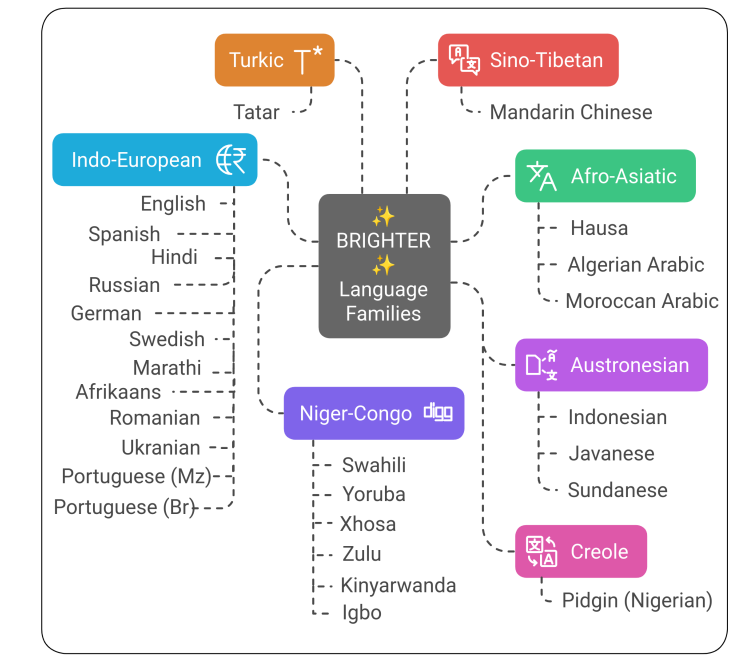
\includegraphics[width=0.5\textwidth]{brighter_languages.png}
    \caption{Languages in BRIGHTER dataset}
    \label{fig:brighter_languages}
\end{figure}

\begin{figure}[h]
    \centering
    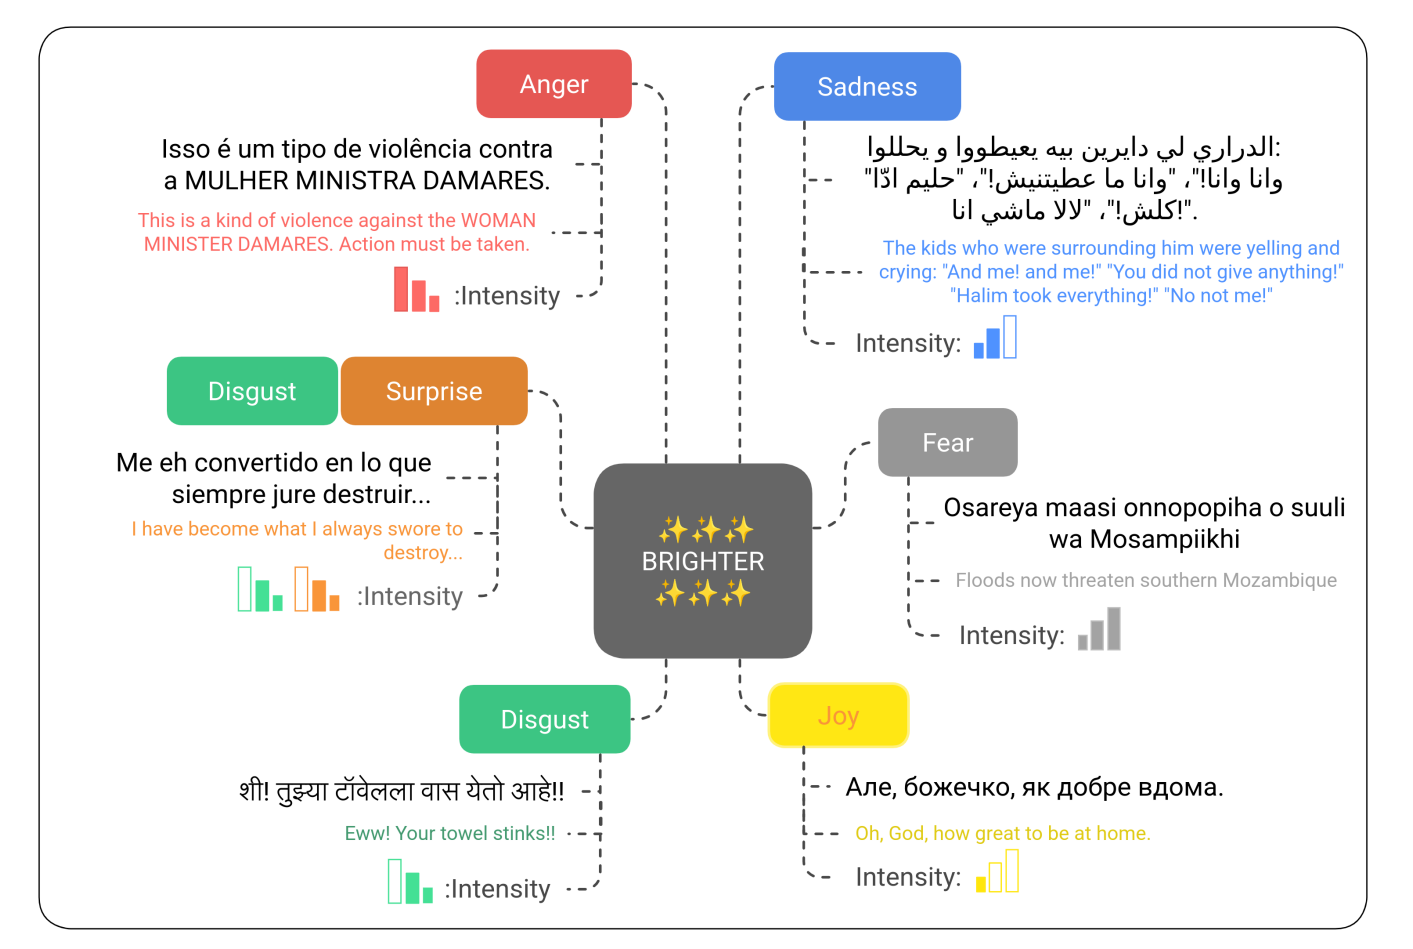
\includegraphics[width=0.8\textwidth]{brighter_examples.png}
    \caption{Examples from BRIGHTER dataset}
    \label{fig:brighter_examples}
\end{figure}

BRIGHTER dataset \cite{muhammad2025brighterbridginggaphumanannotated} is a comprehensive, multi-labeled, multilingual resource for textual emotion recognition, containing more than 100,000 annotated examples across 28 languages and 7 language families. 
BRIGHTER prioritizes low-resource languages from Africa, Asia, Eastern Europe, and Latin America, as these languages are underrepresented in existing datasets.
The dataset also includes mid- and high-resource languages like English, German, and Portuguese.

The collected examples are manually annotated by fluent speakers, 
with six primary perceived emotions — \textit{joy}, \textit{sadness}, \textit{anger}, \textit{fear}, \textit{surprise}, and \textit{disgust}.
If none of these emotions are present, the example is annotated with the \textit{neutral} label.

The dataset collects data from diverse sources, including social media platforms (for example, Reddit, YouTube, Weibo), speeches, literature, news, and even machine-generated examples with human post-editing. 
Examples from the dataset are shown in Figure~\ref{fig:brighter_examples}.
Language family distribution is shown in Figure~\ref{fig:brighter_languages}.

\subsection{Data Splits}
We use the official BRIGHTER dataset splits for all experiments. The Training Set comprises approximately 70\% of the data and is used for supervised model training. The Validation Set, which makes up about 15\% of the data, is utilized for early stopping and hyperparameter tuning. Finally, the Test Set also consists of approximately 15\% of the data and is reserved for final evaluation.

\subsection{Dataset Challenges}

\begin{figure}[h]
    \centering
    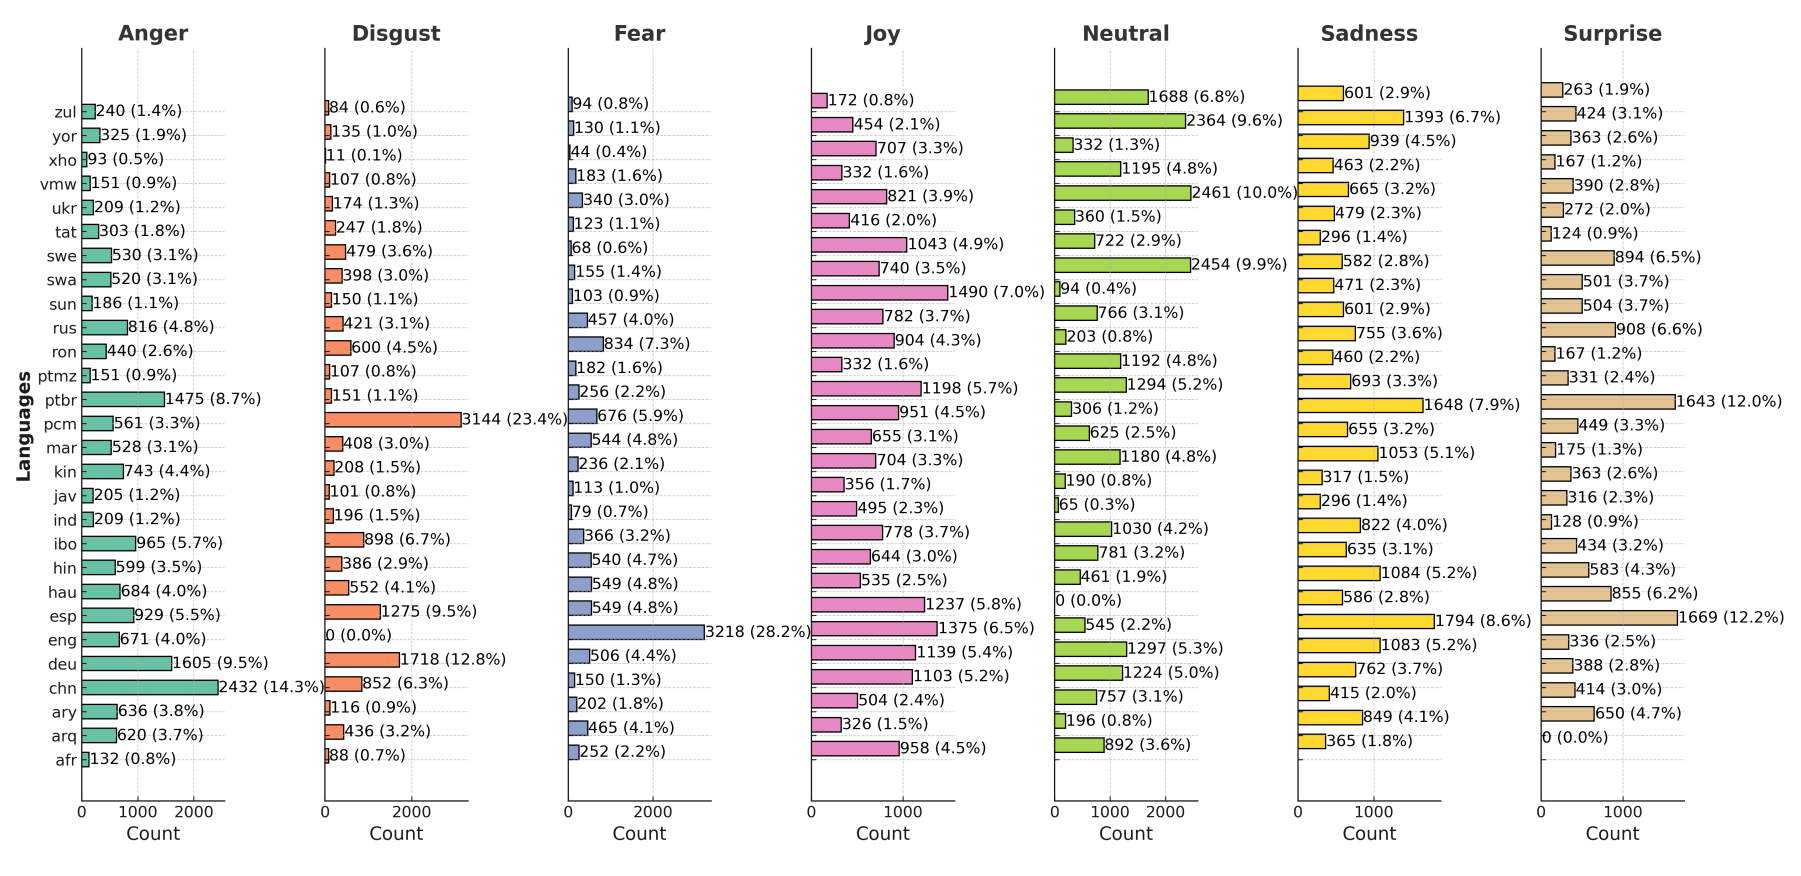
\includegraphics[width=1\textwidth]{brighter_label_distribution.png}
    \caption{Label distribution in the BRIGHTER dataset}
    \label{fig:brighter_label_distribution}
\end{figure}

BRIGHTER introduces several challenges:

Label Distribution: 
The dataset exhibits long-tailed distributions for both emotions and languages, 
as illustrated in Figure~\ref{fig:brighter_label_distribution}. 
Some languages lack examples for certain emotions (e.g., no \textit{disgust} in English, no \textit{surprise} in Afrikaans), and neutral examples vary considerably in frequency.

Linguistic Coverage: BRIGHTER encompasses typologically diverse languages with varying scripts (Latin, Arabic, Devanagari, Cyrillic), making it a robust benchmark for cross-lingual generalization.

\section{Methodology}

We explored four approaches: 

\textbf{BERT-based Approach} fine-tunes a pre-trained model for multi-label prediction, applying a sigmoid function with a 0.5 threshold for binary predictions. It provides a strong baseline but struggles with low-resource languages.

\textbf{Seq2Seq Approach} treats emotion detection as text generation, outputting a list of emotions. It utilizes encoder-decoder models like mT5, BART, and mBART to capture emotion relationships.

\textbf{SetFit Approach} employs few-shot learning with two stages: contrastive learning to fine-tune sentence transformers, and classification using embeddings. It excels with limited data, adapting embeddings for emotion detection.

\textbf{EmoRAG System} leverages retrieval-augmented generation for few-shot learning without parameter updates.
\subsection{BERT-based Approach}

For prediction, we apply a sigmoid function to the model outputs and use a threshold of 0.5 to convert probabilities to binary predictions:

The BERT-based approach provides a strong baseline for emotion detection, leveraging the powerful contextual representations of transformer models. However, it may struggle with low-resource languages where pre-training data is limited.

\subsection{Seq2Seq Approach}

The Seq2Seq approach reframes multi-label emotion detection as a text generation task, where the model generates a comma-separated list of emotions present in the input text. This approach leverages the generative capabilities of encoder-decoder transformer models to directly produce structured outputs rather than independent binary classifications.

This approach is particularly interesting because of the large number of available pre-trained encoder-decoder models.

Some examples of pre-trained encoder-decoder models are:

\textbf{mT5} \cite{xue2021mt5massivelymultilingualpretrained}: A multilingual variant of T5 (Text-to-Text Transfer Transformer) pre-trained on 101 languages. 

\textbf{BART} \cite{lewis2019bartdenoisingsequencetosequencepretraining}: A denoising autoencoder for pretraining sequence-to-sequence models. 

\textbf{mBART} \cite{liu2020multilingualdenoisingpretrainingneural}: A multilingual sequence-to-sequence denoising auto-encoder pre-trained on 25 languages.

The Seq2Seq approach transforms the multi-label classification problem into a text generation task:

\textbf{Input}: The original text to be classified. 

\textbf{Output}: A comma-separated list of emotion labels present in the text (e.g., "joy,surprise,fear").

This format allows the model to learn the relationships between emotions naturally through the generation process, potentially capturing label co-occurrences and dependencies more effectively than independent binary classifiers.

\subsection{SetFit Approach}

SetFit (Sentence Transformer Fine-tuning) is a novel few-shot learning method introduced by \cite{tunstall2022efficient} that combines contrastive learning with standard classification techniques. It was designed to achieve strong performance with limited labeled data, making it particularly suitable for multi-lingual emotion detection where labeled examples may be scarce for low-resource languages.

The SetFit approach involves two stages. 

The first stage is the \textbf{Contrastive Learning Stage}, where a sentence transformer model is fine-tuned using contrastive learning on sentence pairs derived from labeled examples. 

The second stage is the \textbf{Classification Stage}, where a classifier, typically a linear model, is trained on the embeddings produced by the fine-tuned sentence transformer.

Figure~\ref{fig:setfit_training} illustrates the SetFit training process.

\begin{figure}[h]
    \centering
    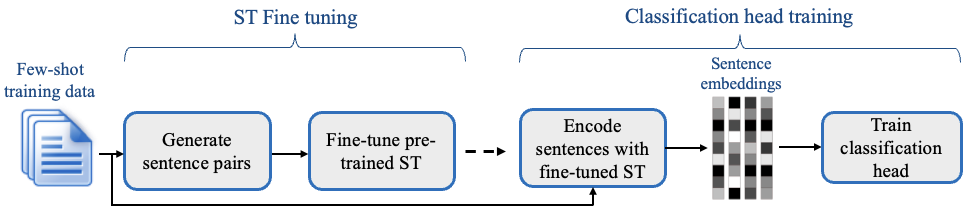
\includegraphics[width=0.8\textwidth]{setfit.png}
    \caption{SetFit training process}
    \label{fig:setfit_training}
\end{figure}

The key innovation of SetFit is its ability to leverage the power of sentence transformers for few-shot learning without requiring extensive labeled data or computationally expensive prompt-based approaches. By fine-tuning the sentence embeddings directly on the task-specific data, SetFit can adapt pre-trained embeddings to better represent the nuances of emotion detection across languages.

\subsection{EmoRAG System}

EmoRAG (Emotion Retrieval-Augmented Generation) is a RAG-based approach to emotion detection.
We retrieve the most similar examples from the labeled dataset and use them as examples for generation with LLMs.

\subsubsection{Pipeline Overview}

EmoRAG architecture follows a four-stage pipeline, shown in Figure~\ref{fig:emorag_pipeline}:

\begin{enumerate}
\item \textbf{Database Construction}: The system indexes labeled examples from the BRIGHTER training dataset as a retrieval corpus.
\item \textbf{Retrieval}: N-gram or embedding-based retriever identifies the top-K most similar examples to a given input.
\item \textbf{Generation}: Retrieved examples are used as few-shot prompts for a set of LLMs to produce emotion predictions.
\item \textbf{Aggregation}: Individual model predictions are combined via an aggregation strategy to produce the final multi-label output.
\end{enumerate}


\begin{figure}[h]
    \centering
    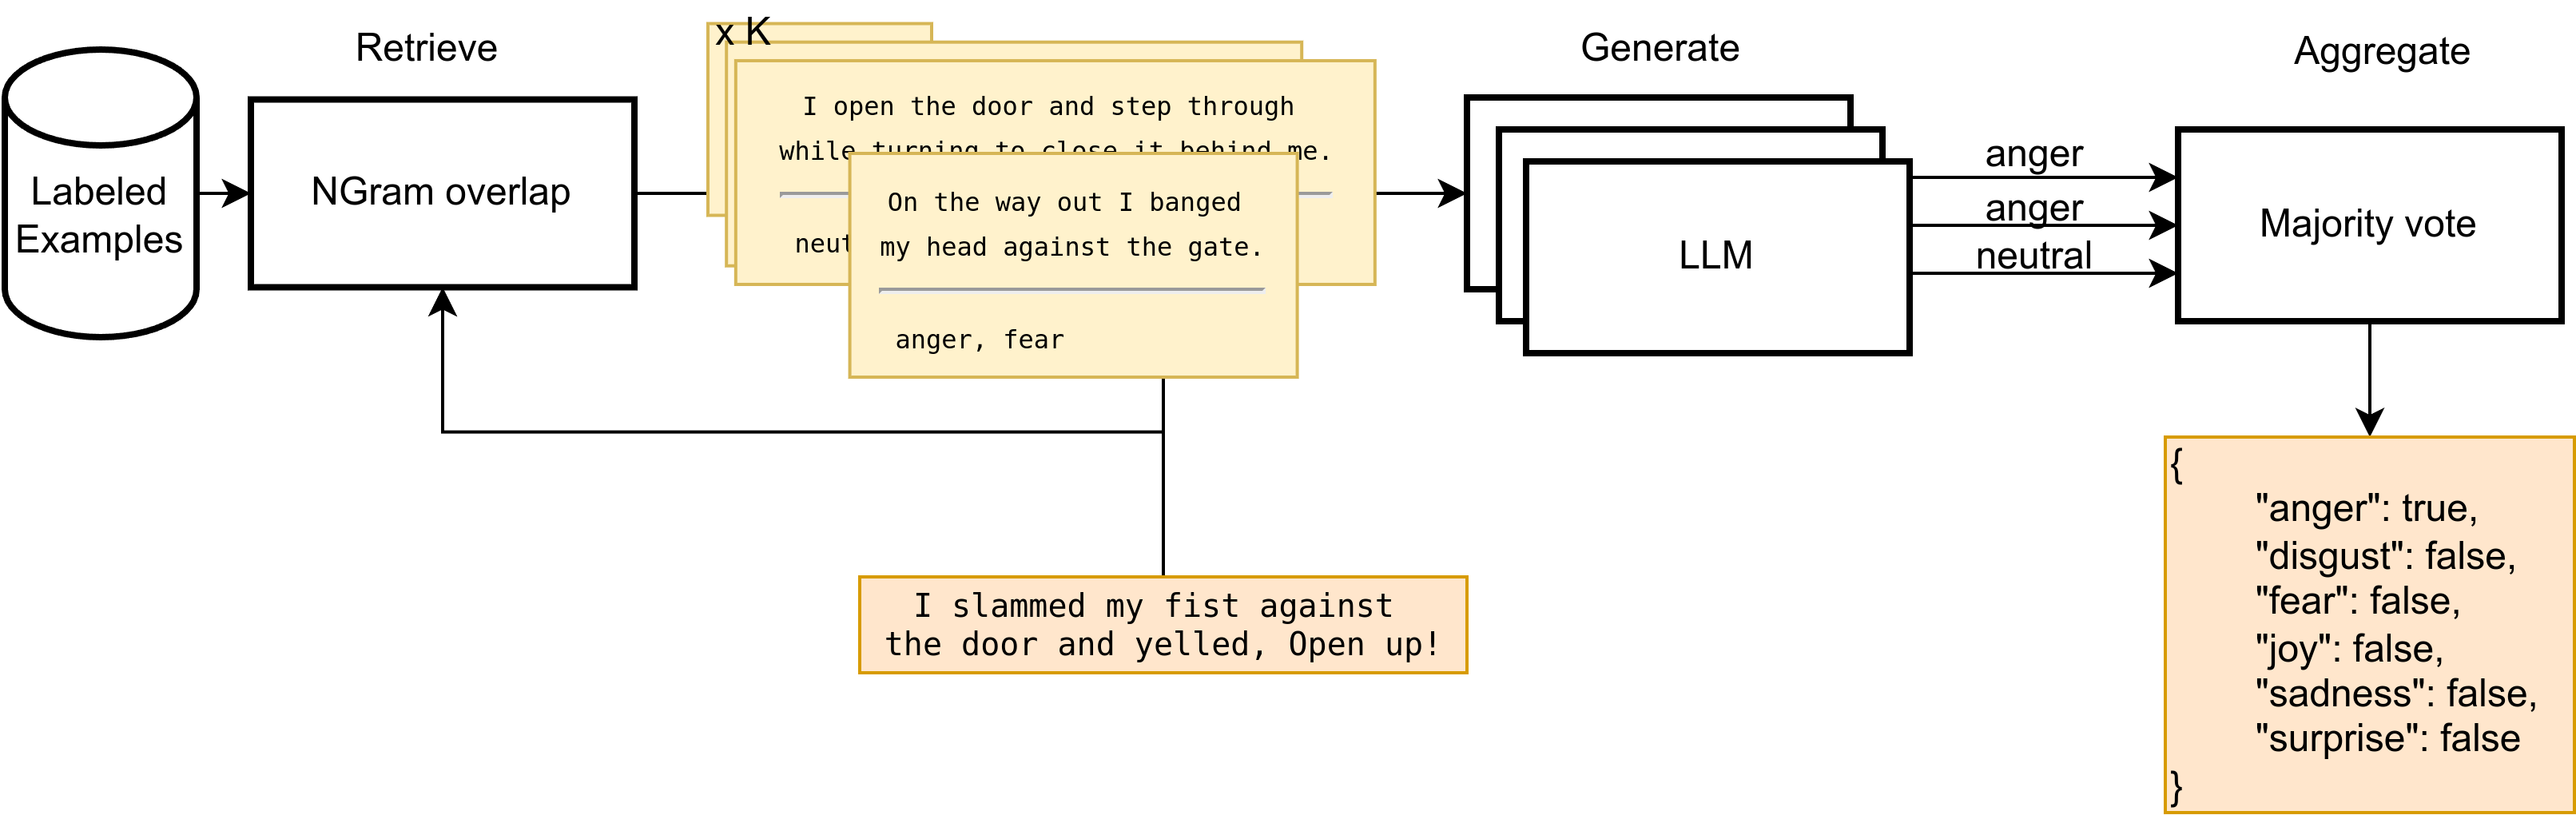
\includegraphics[width=0.8\textwidth]{emorag.png}
    \caption{The diagram of EmoRAG pipeline}
    \label{fig:emorag_pipeline}
\end{figure}

\subsubsection{Retriever Component}

We experimented with two retrieval strategies:


\textbf{N-gram Overlap}: This method retrieves examples based on surface lexical similarity. We have used the n-gram retriever from 
\texttt{LangChain module}~\footnote{\href{https://python.langchain.com/docs/how_to/example_selectors_ngram}{\texttt{python.langchain.com}}}~\cite{Chase_LangChain_2022}. 


\textbf{Embedding-based Retrieval}: Dense vector retriever using sentence-level embeddings that supports multilingual representations. For our experiments, we used the BGE-M3 embedding model \cite{chen2024bgem3embeddingmultilingualmultifunctionality}, which achieved state-of-the-art performance on the multilingual subset of the MTEB benchmark \cite{muennighoff2023mtebmassivetextembedding}.

The number of few-shot samples $K$ is fixed per language type: 30 for low-resource languages and 100 for high-resource ones.

\subsubsection{Generator Models}

For generation, EmoRAG uses diverse ensemble of LLMs including:
\texttt{Llama-3.1-70B \cite{grattafiori2024llama3herdmodels}}, \texttt{Qwen2.5-72B-Instruct \cite{yang2024qwen2technicalreport}}, \texttt{Gemma-2-27B-it \cite{gemmateam2024gemma2improvingopen}}, \texttt{GPT-4o-mini \cite{openai2024gpt4omini}}
Each LLM receives same prompt structure, written in English and formatted to generate emotion predictions in JSON format, as detailed in Appendix~\ref{appendix:llm_prompt}.

\subsubsection{Aggregation Strategies}

To aggregate predictions from multiple LLMs, we evaluate five strategies. 

\textbf{Single model} approach simply uses predictions from one LLM (for example, GPT-4o-mini) without any aggregation. 

\textbf{Majority Vote} gives each model equal vote for each emotion label, with final prediction determined by majority decision (threshold > 0.5). 

In \textbf{Macro/Micro-F1 Weighted Voting}, models' votes are weighted by their macro or micro F1 scores on validation set for specific language, giving more influence to better-performing models. 

\textbf{Label-specific F1 Voting} weights each model's vote by its F1 score for specific emotion label and language, allowing models with higher performance on particular emotions to have more influence on those predictions. 

Finally, \textbf{LLM-based Aggregation} uses one LLM to analyze and aggregate outputs from other models, potentially capturing more nuanced patterns in predictions.

\section{Experiments}

\subsection{Experimental Setup}

Our experiments were conducted in two phases: first, a comprehensive evaluation of all approaches on English data to establish baseline performance, then an extensive multilingual evaluation focusing on our EmoRAG system across all 28 languages in the BRIGHTER dataset.

\subsubsection{Computing Infrastructure}

All experiments were conducted on HSE University's High-Performance Computing (HPC) Cluster "cHARISMa". This infrastructure provided the necessary computational resources for our large-scale experiments, especially for training and evaluating transformer-based models. The cluster includes specialized nodes with NVIDIA Tesla V100 32GB GPUs and newer nodes with NVIDIA A100 80GB GPUs, which were essential for training our larger models. For the most computationally intensive experiments, we used Type C computing nodes equipped with 4 NVIDIA Tesla V100 32GB GPUs with NVLink and 768GB RAM.

\subsubsection{Model Configurations}

For each approach, we used following configurations:

\begin{itemize}
\item \textbf{BERT-based Approach}: We fine-tuned XLM-RoBERTa-large (550M parameters) with classification head for multi-label prediction. Model was initialized with pre-trained weights and fine-tuned on our emotion detection task with learning rate of 2e-5 and batch size of 16.

\item \textbf{SetFit Approach}: We used multilingual MPNet base model as our sentence transformer backbone, with multi-output classification strategy. For few-shot learning, we sampled 8 examples per emotion category, balanced across languages when possible.

\item \textbf{Seq2Seq Approach}: We used mT5-large (1.2B parameters) as our main sequence-to-sequence model, fine-tuned with learning rate of 5e-5 and batch size of 8. We used maximum sequence length of 512 tokens for both input and output.

\item \textbf{EmoRAG System}: Our retrieval component used BGE-M3 embedding model for dense retrieval and n-gram retrieval, with K=30 for low-resource languages and K=100 for high-resource languages. Generator ensemble included Llama-3.1-70B, Qwen2.5-72B-Instruct, Gemma-2-27B-it, and GPT-4o-mini.
\end{itemize}

\subsubsection{Training Process}

Supervised models (BERT, SetFit, Seq2Seq) were trained for 10 epochs with early stopping based on validation loss. BERT and Seq2Seq used the AdamW optimizer, linear learning rate scheduler, and 10\% warmup. SetFit involved contrastive learning and classifier training. EmoRAG required no training, leveraging pre-trained models and retrieval. Training times ranged from 2 hours (SetFit) to 24 hours (Seq2Seq) on the HPC cluster using Slurm.

For English experiments, we evaluated on the validation set, while EmoRAG was assessed on both validation and test sets.

\subsection{Evaluation Metrics}

We used F1-micro and F1-macro for multi-label classification:

F1-micro is calculated by considering all true positives, false positives, and false negatives globally, providing a balance for common labels and high-resource languages.

F1-macro is determined by averaging the F1 scores for each label, making it suitable for datasets with imbalanced label distributions.

\section{Results}

\subsection{English Language}

Table \ref{tab:english_comparison} presents a comprehensive comparison of all methods on the English subset of the BRIGHTER dataset.

\begin{table}[h]
\centering
\begin{tabular}{lcc}
\toprule
\textbf{Method} & \textbf{F1-micro} & \textbf{F1-macro} \\
\midrule
BERT (bert-large-cased) & 0.7145 & 0.6468 \\
SetFit (bge-m3) & 0.6943 & 0.5591 \\
Seq2Seq (bart-large-cnn) & 0.5126 & 0.4566 \\
GPT-4 (zero-shot) & 0.5959 & 0.6164 \\
\midrule
\multicolumn{3}{c}{\textbf{EmoRAG Variants}} \\
\midrule
Llama-3.1-70B (few-shot, bge-m3) & 0.7499 & 0.7239 \\
Qwen2.5 (few-shot, bge-m3) & 0.7790 & 0.7749 \\
GPT-4o-mini (few-shot, bge-m3) & 0.8071 & 0.8026 \\
GPT-4o-mini (few-shot, ngram) & 0.7810 & 0.7700 \\
EmoRAG (majority vote) & 0.8080 & 0.8010 \\
EmoRAG (majority vote macro) & 0.8130 & 0.8100 \\
EmoRAG (label-specific F1) & \textbf{0.8210} & \textbf{0.8180} \\
\bottomrule
\end{tabular}
\caption{Performance comparison of different approaches on English language subset of validation set}
\label{tab:english_comparison}
\end{table}

EmoRAG system with label-specific F1 weighting achieved the highest performance, with an F1 micro score of 0.821 and an F1 macro score of 0.818, significantly outperforming all other approaches. Among traditional supervised methods, BERT performed best with 0.7145 F1 micro, followed by SetFit at 0.6943. The Seq2Seq approach showed the weakest performance among the supervised methods, with an F1-micro of only 0.5126.

Notably, all EmoRAG variants outperformed supervised approaches, with even a single-model GPT-4o-mini achieving an F1-micro of 0.8071, demonstrating the effectiveness of retrieval-augmented generation for this task. Ensemble-based aggregation strategies further improved performance, with label-specific F1 weighting yielding the best results.

Regarding efficiency, supervised approaches required extensive training time (24 hours for Seq2Seq, 8 hours for BERT, and 2 hours for SetFit on our hardware), while EmoRAG did not require training but incurred higher inference costs due to multiple LLM calls. The average inference time per sample was 0.05 seconds for BERT, 0.12 seconds for SetFit, 0.3 seconds for Seq2Seq, and 2.5 seconds for EmoRAG with four models.

\subsection{All Languages}

\begin{figure}[h]
    \centering
    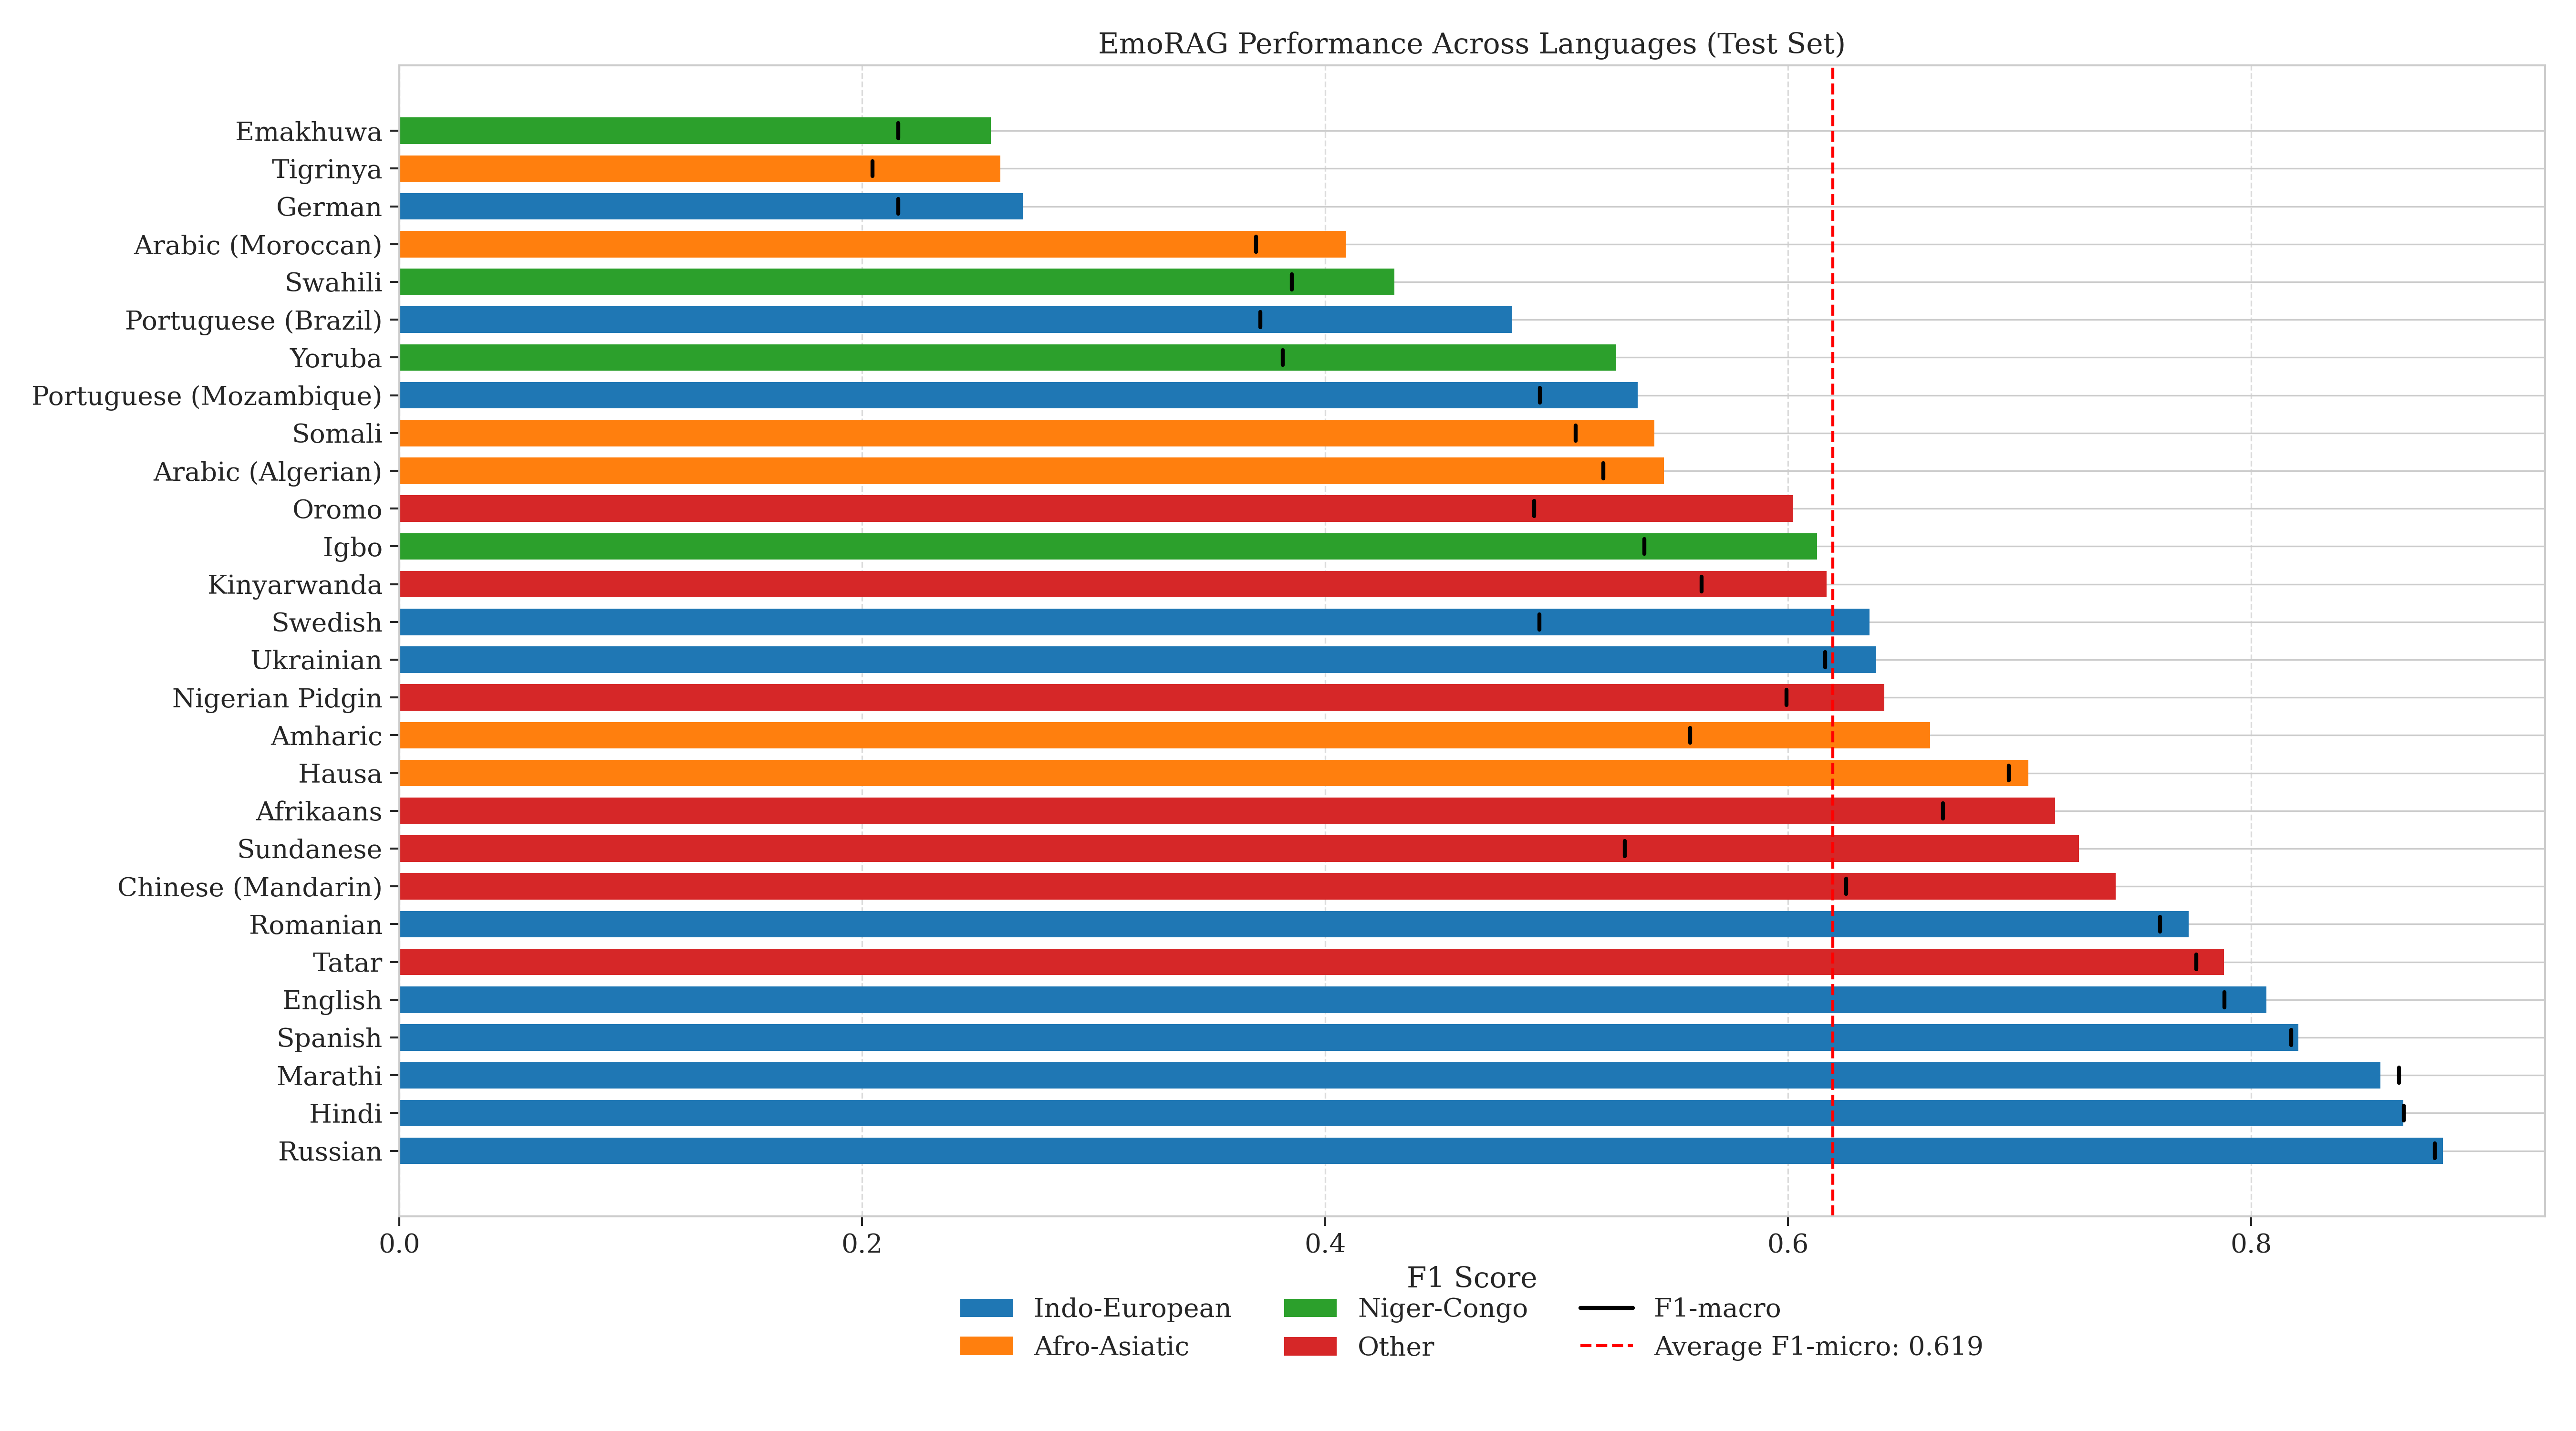
\includegraphics[width=1\textwidth]{emorag_by_language.png}
    \caption{EmoRAG performance across all 28 languages in BRIGHTER dataset}
    \label{fig:emorag_by_language}
\end{figure}


Table \ref{tab:multilingual_performance} presents the performance of our best EmoRAG system in all 28 languages in the BRIGHTER dataset in the validation set, showing F1-micro/F1-macro scores for each language and the aggregation method.

Table \ref{tab:test_metrics} presents the performance of our best EmoRAG system in all 28 languages in the BRIGHTER dataset in the test set, showing F1-micro/F1-macro scores for each language and the aggregation method.

Figure \ref{fig:emorag_by_language} shows performance of our best EmoRAG system across all 28 languages in BRIGHTER dataset on validation set, showing F1-micro/F1-macro scores for best performing model for each language.

\begin{table*}[!th]
\begin{center}
    
    \footnotesize
    \resizebox{\textwidth}{!}{
    \begin{tabular}{@{}lccccccccc@{}}
    \toprule
    \textbf{Language} & \textbf{llama-3.1-70b} & \textbf{qwen2.5-70b} & \textbf{gpt-4o-mini} & \textbf{gpt-4o-mini-ngram} & \textbf{gemma29b} & \textbf{gemma29b\_ngram} & \textbf{majority\_vote} & \textbf{majority\_vote\_macro} & \textbf{majority\_vote\_by\_label\_f1} \\ \midrule
    amh & 0.534/0.448 & - & \textbf{0.637/0.503} & 0.633/0.493 & 0.609/0.488 & 0.582/0.474 & 0.659/0.535 & 0.659/0.535 & 0.655/0.539 \\
    arq & 0.584/0.575 & 0.623/0.597 & 0.613/0.596 & \textbf{0.663/0.655} & 0.614/0.589 & 0.578/0.531 & 0.645/0.615 & 0.653/0.665 & 0.687/0.677 \\
    ary & 0.542/0.490 & 0.540/0.485 & 0.552/0.499 & \textbf{0.576/0.512} & 0.575/0.521 & 0.584/0.484 & 0.607/0.526 & 0.526/0.599 & 0.616/0.540 \\
    afr & 0.560/0.444 & \textbf{0.629/0.527} & 0.662/0.567 & 0.646/0.572 & 0.584/0.481 & 0.484/0.398 & 0.601/0.494 & 0.546/0.646 & 0.662/0.557 \\
    chn & 0.676/0.603 & 0.589/0.570 & 0.698/0.579 & \textbf{0.748/0.604} & 0.693/0.572 & 0.709/0.543 & 0.749/0.642 & 0.652/0.757 & 0.759/0.659 \\
    deu & 0.745/0.588 & 0.521/0.499 & \textbf{0.745/0.694} & 0.738/0.662 & 0.632/0.559 & 0.659/0.593 & 0.738/0.659 & 0.672/0.741 & 0.752/0.695 \\
    eng & 0.735/0.726 & 0.779/0.775 & 0.807/0.803 & 0.770/0.781 & 0.769/0.759 & 0.720/0.723 & 0.801/0.808 & 0.813/0.810 & \textbf{0.821/0.818} \\
    esp & 0.751/0.744 & 0.788/0.778 & 0.793/0.785 & 0.799/0.793 & 0.778/0.772 & 0.782/0.778 & 0.786/0.778 & 0.807/0.812 & \textbf{0.813/0.809} \\
    hau & 0.610/0.602 & 0.607/0.598 & 0.669/0.662 & \textbf{0.696/0.687} & 0.682/0.676 & 0.698/0.689 & 0.735/0.728 & 0.734/0.738 & 0.735/0.731 \\
    hin & 0.780/0.791 & 0.707/0.728 & 0.805/0.803 & 0.811/0.812 & 0.796/0.799 & 0.798/0.806 & 0.838/0.842 & 0.833/0.830 & \textbf{0.842/0.849} \\
    ibo & 0.531/0.486 & 0.502/0.452 & 0.572/0.514 & 0.564/0.499 & 0.574/0.508 & 0.574/0.520 & 0.609/0.532 & 0.534/0.608 & \textbf{0.614/0.550} \\
    kin & 0.443/0.385 & 0.443/0.382 & 0.555/0.491 & \textbf{0.576/0.489} & 0.477/0.404 & 0.514/0.466 & 0.589/0.515 & 0.501/0.570 & 0.575/0.512 \\
    mar & 0.874/0.883 & 0.904/0.908 & 0.937/0.939 & 0.937/0.939 & 0.883/0.883 & 0.897/0.900 & 0.942/0.946 & 0.935/0.931 & \textbf{0.943/0.947} \\
    orm & 0.467/0.369 & 0.521/0.415 & 0.552/0.455 & \textbf{0.607/0.501} & 0.519/0.404 & 0.488/0.362 & 0.585/0.446 & 0.493/0.608 & 0.608/0.488 \\
    pcm & 0.532/0.508 & 0.573/0.535 & 0.599/0.542 & \textbf{0.628/0.573} & 0.608/0.572 & 0.585/0.548 & 0.621/0.574 & 0.590/0.633 & 0.638/0.591 \\
    ptbr & 0.686/0.547 & 0.662/0.569 & 0.731/0.633 & 0.707/0.603 & 0.726/0.617 & 0.710/0.525 & 0.766/0.626 & 0.658/0.760 & \textbf{0.766/0.645} \\
    ptmz & 0.454/0.456 & 0.539/0.532 & 0.515/0.484 & 0.478/0.443 & 0.521/0.486 & 0.494/0.445 & 0.565/0.558 & 0.543/0.552 & \textbf{0.565/0.558} \\
    ron & 0.758/0.749 & 0.745/0.726 & 0.756/0.741 & 0.778/0.763 & 0.745/0.719 & 0.754/0.724 & 0.773/0.751 & 0.771/0.790 & \textbf{0.794/0.774} \\
    rus & 0.835/0.836 & 0.861/0.857 & 0.839/0.833 & 0.812/0.806 & 0.841/0.834 & 0.824/0.817 & 0.879/0.877 & 0.881/0.883 & \textbf{0.880/0.880} \\
    som & 0.361/0.296 & 0.379/0.338 & 0.518/0.469 & 0.528/0.491 & 0.426/0.381 & 0.428/0.382 & 0.494/0.420 & 0.464/0.514 & \textbf{0.519/0.477} \\
    sun & 0.674/0.496 & 0.707/0.491 & 0.734/0.596 & 0.757/0.612 & 0.708/0.532 & 0.733/0.565 & 0.754/0.537 & 0.564/0.750 & \textbf{0.757/0.614} \\
    swa & 0.357/0.329 & 0.376/0.345 & 0.391/0.366 & 0.416/0.401 & 0.401/0.366 & 0.407/0.372 & 0.435/0.396 & 0.401/0.435 & \textbf{0.440/0.409} \\
    swe & 0.684/0.475 & 0.680/0.502 & 0.709/0.528 & 0.708/0.529 & 0.699/0.518 & 0.671/0.501 & 0.734/0.555 & 0.547/0.727 & \textbf{0.736/0.582} \\
    tat & 0.652/0.611 & 0.663/0.631 & 0.712/0.671 & 0.702/0.660 & 0.669/0.634 & 0.637/0.592 & 0.727/0.673 & 0.688/0.732 & \textbf{0.749/0.710} \\
    tir & - & - & 0.377/0.321 & 0.384/0.319 & - & - & 0.322/0.263 & 0.321/0.377 & \textbf{0.397/0.342} \\
    ukr & 0.521/0.512 & 0.601/0.579 & 0.581/0.567 & 0.550/0.537 & 0.587/0.553 & 0.535/0.469 & 0.622/0.611 & 0.621/0.625 & \textbf{0.634/0.621} \\
    vmw & 0.158/0.145 & 0.261/0.184 & 0.300/0.211 & 0.226/0.158 & 0.246/0.206 & 0.186/0.159 & 0.190/0.140 & 0.180/0.230 & \textbf{0.257/0.205} \\
    yor & 0.354/0.255 & 0.415/0.300 & 0.474/0.374 & 0.506/0.420 & 0.436/0.317 & 0.472/0.347 & 0.564/0.443 & 0.423/0.532 & \textbf{0.564/0.443} \\ \midrule
    \textbf{Average} & \textbf{0.563/0.515} & \textbf{0.590/0.556} & \textbf{0.631/0.590} & \textbf{0.641/0.601} & \textbf{0.617/0.576} & \textbf{0.607/0.566} & \textbf{0.661/0.617} & \textbf{0.646/0.634} & \textbf{0.678/0.634} \\ \bottomrule
    \end{tabular}
    }
\end{center}
\caption{Development set F1-micro/F1-macro scores for each language and model. The best model for each language is highlighted in bold.}
\label{tab:multilingual_performance}
\end{table*}

\begin{table*}[th!]
\centering
\footnotesize

\resizebox{.99\textwidth}{!}{

\begin{tabular}{@{}lcccccc@{}}
\toprule
\textbf{Language} & \textbf{Language Code} & \textbf{Best Model} & \textbf{Dev F1 Micro} & \textbf{Dev F1 Macro} & \textbf{Test F1 Micro} & \textbf{Test F1 Macro} \\ \midrule
Afrikaans & afr & majority\_vote\_by\_label\_f1 & 0.662 & 0.557 & 0.7153 & 0.667 \\
Amharic & amh & gpt-4o-mini & 0.637 & 0.503 & 0.6613 & 0.5578 \\
German & deu & gpt-4o-mini & 0.745 & 0.694 & 0.2694 & 0.2156 \\
English & eng & majority\_vote\_by\_label\_f1 & 0.821 & 0.818 & 0.8066 & 0.7885 \\
Spanish & esp & majority\_vote\_by\_label\_f1 & 0.813 & 0.809 & 0.8204 & 0.8174 \\
Hindi & hin & majority\_vote\_by\_label\_f1 & 0.842 & 0.849 & 0.8658 & 0.8661 \\
Marathi & mar & majority\_vote\_by\_label\_f1 & 0.943 & 0.947 & 0.8559 & 0.864 \\
Oromo & orm & gpt-4o-mini-ngram & 0.607 & 0.501 & 0.6023 & 0.4903 \\
Portuguese (Brazil) & ptbr & majority\_vote\_by\_label\_f1 & 0.766 & 0.645 & 0.4809 & 0.372 \\
Russian & rus & majority\_vote\_by\_label\_f1 & 0.880 & 0.880 & 0.8829 & 0.8794 \\
Somali & som & majority\_vote\_by\_label\_f1 & 0.519 & 0.477 & 0.5422 & 0.5082 \\
Sundanese & sun & gpt-4o-mini-ngram & 0.757 & 0.612 & 0.7256 & 0.5294 \\
Tatar & tat & majority\_vote\_by\_label\_f1 & 0.749 & 0.710 & 0.7884 & 0.7763 \\
Tigrinya & tir & majority\_vote\_by\_label\_f1 & 0.397 & 0.342 & 0.2597 & 0.2044 \\
Arabic (Algerian) & arq & majority\_vote\_by\_label\_f1 & 0.687 & 0.677 & 0.5464 & 0.5203 \\
Arabic (Moroccan) & ary & gpt-4o-mini-ngram & 0.576 & 0.512 & 0.4089 & 0.3701 \\
Chinese (Mandarin) & chn & gpt-4o-mini-ngram & 0.748 & 0.604 & 0.7416 & 0.6252 \\
Hausa & hau & majority\_vote\_by\_label\_f1 & 0.735 & 0.731 & 0.7039 & 0.6954 \\
Kinyarwanda & kin & gpt-4o-mini-ngram & 0.576 & 0.489 & 0.6167 & 0.5627 \\
Nigerian Pidgin & pcm & majority\_vote\_by\_label\_f1 & 0.638 & 0.591 & 0.6416 & 0.5993 \\
Portuguese (Mozambique) & ptmz & majority\_vote\_by\_label\_f1 & 0.565 & 0.558 & 0.535 & 0.4927 \\
Swahili & swa & majority\_vote\_by\_label\_f1 & 0.440 & 0.409 & 0.43 & 0.3856 \\
Swedish & swe & majority\_vote\_by\_label\_f1 & 0.736 & 0.582 & 0.6353 & 0.4926 \\
Ukrainian & ukr & majority\_vote\_by\_label\_f1 & 0.634 & 0.621 & 0.638 & 0.6161 \\
Emakhuwa & vmw & gpt-4o-mini & 0.300 & 0.211 & 0.2556 & 0.2157 \\
Yoruba & yor & majority\_vote\_by\_label\_f1 & 0.564 & 0.443 & 0.5257 & 0.3818 \\
Igbo & ibo & majority\_vote\_by\_label\_f1 & 0.614 & 0.550 & 0.6125 & 0.5379 \\
Romanian & ron & majority\_vote\_by\_label\_f1 & 0.794 & 0.774 & 0.773 & 0.7608 \\ \midrule
\textbf{Average} & & & & & \textbf{0.638} & \textbf{0.590} \\ \bottomrule
\end{tabular}
}
\caption{Test set performance metrics for each language using the best model according to the development dataset results.}
\label{tab:test_metrics}
\end{table*}


We have identified several key patterns in the performance of EmoRAG.

High-resource languages such as English, Russian, and Hindi consistently achieved superior results, with F1-micro scores above 0.8. 
Low-resource languages like Tigrinya, Swahili, and Makhuwa exhibited significantly lower performance, with F1-micro scores below 0.5.
Indo-European languages generally performed above average, with F1-micro scores around 0.795. 
Niger-Congo  and Afro-Asiatic languages generally performed below average, with F1-micro scores around 0.563. 
The retrieval strategy also impacted performance; n-gram retrieval was more effective than embedding-based retrieval for languages with unique scripts or limited pre-training data representation, as seen in Oromo, Moroccan Arabic, and Chinese. Furthermore, the label-specific F1 weighting strategy was the most effective aggregation method, outperforming others in 17 out of 28 languages, indicating that emotion-specific expertise varies across models and languages.


\section{Ablation Studies}

To understand the contribution of different components to EmoRAG's performance, we conducted extensive ablation studies.

\subsection{EmoRAG Components}

\begin{table}[h]
\centering
\begin{tabular}{lcc}
\toprule
\textbf{Component Configuration} & \textbf{F1-micro} & \textbf{F1-macro} \\
\midrule
Full EmoRAG system & 0.678 & 0.634 \\
Without embedding retriever & 0.641 & 0.601 \\
Without n-gram retriever & 0.631 & 0.590 \\
Without label-specific weighting & 0.661 & 0.617 \\
Single model (GPT-4o-mini) & 0.631 & 0.590 \\
\bottomrule
\end{tabular}
\caption{Ablation study of EmoRAG components (averaged across all languages)}
\label{tab:ablation_components}
\end{table}

Removing the embedding-based retriever led to a 5.5\% drop in performance on average, affecting high-resource languages more severely. Removing the n-gram retriever caused a smaller drop of 6.9\%, but it had a significant impact on low-resource languages with unique scripts. Using label-specific weighting improved results by 2.6\% compared to simple majority voting, especially in languages where emotion distribution is uneven.

\subsection{Example Count Analysis}

% \begin{figure}[h]
%     \centering
%     \includegraphics[width=0.8\textwidth]{example_count_analysis.png}
%     \caption{Performance vs. number of retrieved examples}
%     \label{fig:example_count}
% \end{figure}

We varied the number of retrieved examples (K) from 0 to 1000 and found that performance generally improved with more examples up to a point, after which returns diminished or performance decreased. The optimal K varied by language: high-resource languages benefited from larger K values (100-150), while low-resource languages performed best with moderate K values (30-50). This suggests that the quality of examples matters more than quantity for low-resource settings.

\begin{table}[h]
\centering
\begin{tabular}{lcc}
\toprule
\textbf{Number of Examples (K)} & \textbf{F1-micro} & \textbf{F1-macro} \\
\midrule
0 (zero-shot) & 0.5959 & 0.6164 \\
30 & 0.8036 & 0.8001 \\
100 & 0.8071 & 0.8026 \\
300 & 0.7911 & 0.7762 \\
1000 & 0.7882 & 0.7769 \\
\bottomrule
\end{tabular}
\caption{Impact of retrieved example count on GPT-4o-mini performance for English language}
\label{tab:example_count}
\end{table}

As shown in Table \ref{tab:example_count}, for English, performance improves dramatically when moving from zero-shot to few-shot with 30 examples, with a slight additional improvement at 100 examples. However, increasing to 300 or 1000 examples actually leads to decreased performance. This pattern suggests that there is an optimal window for the number of retrieved examples.

\subsection{Cross-model Analysis}

\begin{table}[h]
\centering
\begin{tabular}{lcc}
\toprule
\textbf{Model} & \textbf{F1-micro} & \textbf{F1-macro} \\
\midrule
GPT-4o-mini & 0.631 & 0.590 \\
Llama-3.1-70B & 0.649 & 0.612 \\
Qwen2.5-72B & 0.657 & 0.621 \\
Gemma-2-27B & 0.618 & 0.583 \\
All models (ensemble) & 0.678 & 0.634 \\
\bottomrule
\end{tabular}
\caption{Performance comparison across different LLMs (averaged across all languages)}
\label{tab:cross_model}
\end{table}

Each model within our ensemble demonstrated distinct strengths across various languages and emotional categories. 
The Llama-3.1-70B model showed outstanding performance in Germanic and Romance languages. 
In contrast, the Qwen2.5-72B model was particularly effective in Asian languages. 
The GPT-4o-mini model delivered more consistent performance across all language categories. 
Gemma-2-27B was especially effective in predicting emotions like surprise and fear within Slavic languages.

The ensemble consistently outperformed individual models, with an average improvement of 3.2\% in F1-micro score over the best single model. 
This confirms the complementary nature of different LLMs' knowledge.

\section{Discussion}

Our experiments on multi-lingual, multi-label emotion detection reveal key insights into each method's strengths and weaknesses, with broader implications for cross-language emotion detection.

\subsection{Comparative Analysis of Approaches}

Retrieval-augmented generation methods outperform traditional supervised learning. EmoRAG consistently surpasses BERT, SetFit, and Seq2Seq models, especially in low-resource languages.

\textbf{BERT-based Approach}: BERT provides a strong baseline (F1-micro of 0.7145 on English) but struggles with low-resource languages due to limited pre-training data. Its binary relevance method may not capture emotion label connections, and extensive fine-tuning is data-intensive.

\textbf{SetFit Approach}: SetFit (F1-micro of 0.6943 on English) is promising for few-shot learning but lags behind EmoRAG. Its two-stage training uses limited data well, but contrastive learning may miss emotional nuances. It is efficient when resources are scarce.

\textbf{Seq2Seq Approach}: Seq2Seq, despite its potential for label dependency, performs weakest (F1-micro of 0.5126 on English). Treating emotion detection as a generation task adds complexity without clear benefits, especially for texts with multiple emotions.

\textbf{EmoRAG System}: EmoRAG excels (F1-micro of 0.8210 on English) by leveraging training data at inference without extensive fine-tuning. Powerful LLMs enable contextual emotion reasoning, and ensemble label-specific weighting combines model strengths.

\subsection{Cross-lingual Performance}

EmoRAG's performance across 28 languages shows:

\textbf{High-resource vs. Low-resource Languages}: EmoRAG performs better on high-resource languages (e.g., English, German, Spanish) with a smaller performance gap than supervised methods. It achieves competitive results in some low-resource languages (e.g., Amharic, Algerian Arabic), indicating effective cross-language knowledge transfer.

\textbf{Script and Typological Factors}: Non-Latin script languages (e.g., Arabic, Amharic, Hindi) show lower performance than Latin scripts, but the gap is less than with supervised methods, suggesting EmoRAG's retrieval can bridge typological differences.

\textbf{Retrieval Strategy Impact}: Embedding-based retrieval outperforms n-gram retrieval in high-resource languages. In some low-resource languages with limited embedding model pre-training data, n-gram retrieval is more effective, highlighting the need for language-specific retrieval strategies.

\subsection{Examples of emotion intensity confusion}

Analysis of misclassifications reveals several common error patterns across approaches, which can be illustrated through specific examples from our evaluation dataset:

\textbf{Emotion Intensity Confusion:} All approaches struggled with distinguishing between different intensities of the same emotion. For example, as shown in Table~\ref{tab:intensity-confusion}:

\begin{table}[h]
\centering
\begin{tabular}{|p{8.5cm}|p{2.5cm}|p{2.5cm}|}
\hline
\textbf{Text} & \textbf{True Emotions} & \textbf{Predicted Emotions} \\
\hline
``Ich wurde mit 17 ins Milieu verschleppt, gehandelt, verkauft, zur einer Schwangerschaft (und Austragung) gezwungen und konnte erst mit fast 20 flüchten. Gemeinsam mit meinem Kind.'' \newline (German: "I was abducted into prostitution at 17, trafficked, sold, forced into pregnancy (and carrying to term) and could only escape at almost 20. Together with my child.") & anger, disgust, sadness & anger, disgust, fear, sadness \\
\hline
``Taurus-Leaks: Der Skandal besteht darin, dass deutsche Offiziere mit deutschen Waffen einen Angriff gegen Russland bis ins Detail planen.'' \newline (German: "Taurus Leaks: The scandal is that German officers are planning an attack against Russia with German weapons in detail.") & anger, disgust, fear & anger, disgust, fear, surprise \\
\hline
\end{tabular}
\caption{Examples of emotion intensity confusion}
\label{tab:intensity-confusion}
\end{table}

In these examples, the model correctly identified the primary emotions but added additional emotions that weren't annotated, suggesting difficulty in calibrating emotional intensity thresholds.

\textbf{Cultural Nuances:} Expressions that rely on cultural context or idioms were frequently misclassified, as illustrated in Table~\ref{tab:cultural-nuances}:

\begin{table}[h]
\centering
\begin{tabular}{|p{8.5cm}|p{2.5cm}|p{2.5cm}|}
\hline
\textbf{Text} & \textbf{True Emotions} & \textbf{Predicted Emotions} \\
\hline
``@<username> @<username> Jack na akpari onwe ya'' \newline (Igbo: "Jack is just boasting") & anger & [none] \\
\hline
``Anu Matak Mun di Imah kosong tong ngomong punten bisi Aya NU nembalan'' \newline (Sundanese: "Why do we say 'excuse me' in an empty house? In case someone answers") & fear & fear, surprise \\
\hline
``Vi blev någorlunda nöjda. Vi kommenterade missnöjet, en väldigt liten åtgärd gjordes men ändock blev vi inte helt nöjda.'' \newline (Swedish: "We were somewhat satisfied. We commented on the dissatisfaction, a very small measure was taken but still we were not completely satisfied.") & joy & anger, sadness \\
\hline
\end{tabular}
\caption{Examples of cultural nuance misclassifications}
\label{tab:cultural-nuances}
\end{table}

These examples demonstrate how culturally-specific expressions of emotions can be misinterpreted, particularly in low-resource languages where models have less exposure to cultural nuances.

\textbf{Co-occurring Emotions:} Cases where multiple emotions co-occur presented challenges, as shown in Table~\ref{tab:co-occurring-emotions}:

\begin{table}[h]
\centering
\begin{tabular}{|p{8.5cm}|p{2.5cm}|p{2.5cm}|}
\hline
\textbf{Text} & \textbf{True Emotions} & \textbf{Predicted Emotions} \\
\hline
``It overflowed and brown shitty diarrhea water came flooding under the stall wall into my wife's stall.'' & anger, fear, sadness, surprise & anger, fear, surprise \\
\hline
``Caz halucinant de cruzime Un bărbat acuză un polițist din Sibiu că la snopit în bătaie "Am stat în genunchi"'' \newline (Romanian: "Hallucinating case of cruelty A man accuses a police officer from Sibiu of beating him up 'I was on my knees'") & anger, disgust, fear, sadness, surprise & anger, disgust, sadness \\
\hline
``Pobre chica, te quemaste tu solita.'' \newline (Spanish: "Poor girl, you burned yourself.") & disgust, sadness, surprise & sadness \\
\hline
\end{tabular}
\caption{Examples of co-occurring emotion misclassifications}
\label{tab:co-occurring-emotions}
\end{table}

These examples show that models often capture the dominant emotions but miss secondary or tertiary emotions, particularly in complex emotional scenarios.

\textbf{Linguistic Structure:} Languages with significantly different syntactic structures showed higher error rates, as demonstrated in Table~\ref{tab:linguistic-structure}:

\begin{table}[h]
\centering
\begin{tabular}{|p{8.5cm}|p{2.5cm}|p{2.5cm}|}
\hline
\textbf{Text} & \textbf{True Emotions} & \textbf{Predicted Emotions} \\
\hline
``[Tigrinya text omitted]'' \newline (Tigrinya expression of disgust) & disgust & [none] \\
\hline
``[Makhuwa text omitted]'' \newline (Makhuwa: "Brazil is now the father of the World Cup and looks weak.") & sadness & [none] \\
\hline
``[Chinese text omitted]'' \newline (Chinese: "Sigh, people can't see that he's still the pill king, don't know where he got the money from, I'm short on cash recently and would like to earn some too.") & [none] & anger \\
\hline
\end{tabular}
\caption{Examples of linguistic structure challenges}
\label{tab:linguistic-structure}
\end{table}

These examples highlight the challenges in processing languages with different scripts and syntactic structures, particularly for low-resource languages where pre-training data is limited.

\section{Conclusions}

This thesis has investigated various approaches for multilingual, multi-label emotion detection, with particular focus on addressing challenges of low-resource languages. We compared traditional supervised approaches (BERT, SetFit, and Seq2Seq) with a novel retrieval-augmented generation system (EmoRAG). We have evaluated our system on 28 languages from the BRIGHTER dataset.

\subsection{Summary of Findings}

Our research has yielded several key findings:

\begin{itemize}
    \item Retrieval-augmented generation significantly performs better than traditional supervised approaches for emotion detection on English.
    
    \item Performance gap between high-resource and low-resource languages still remains substantial.
    
    \item Different retrieval strategies are optimal for different languages: embedding-based retrieval works best for high-resource languages with substantial pre-training data, while n-gram retrieval often performs better for languages with unique scripts or limited representation in pre-training.
    
    \item Ensemble methods that combine predictions from multiple models with label-specific weighting strategies consistently performed better than single-model approaches, demonstrating complementary nature of different LLMs' capabilities across languages and emotions.
    
\end{itemize}

\subsection{Limitations}

Despite promising results, our approaches face several limitations:

\begin{itemize}
    \item Performance on Very Low-Resource Languages: Even with retrieval augmentation, performance on extremely low-resource languages like Makhuwa (F1-micro of 0.257) and Tigrinya (F1-micro of 0.397) remained poor, indicating that fundamental challenges in cross-lingual transfer persist.
    
    \item Cultural Nuance: All approaches struggled with culturally-specific expressions of emotion, particularly idioms and metaphorical language that require cultural context to interpret correctly.
    
    \item Retrieval Quality: The effectiveness of retrieval-augmented approaches depends heavily on the quality and relevance of retrieved examples. Current retrieval mechanisms do not account for cultural or pragmatic factors that influence emotion expression.
    
\end{itemize}


In conclusion, while there are still challenges in detecting emotions across multiple languages, especially those with fewer resources, our research shows that using retrieval-augmented methods is a promising way forward. By leveraging the capabilities of large language models and flexible retrieval techniques, we can create systems that better understand emotions in different cultural contexts.

Our EmoRAG system participated in the SemEval2025-Task11 competition, ranking in the top 10 on average across all languages, with some languages achieving top 3 performance. 

The EmoRAG system description paper was accepted at ACL Workshop 2025.

We have made our complete implementation publicly available at \url{https://github.com/galthran-wq/semeval25-text-emotions}. This repository includes code for all components of the EmoRAG system and complete implementation of all approaches tested in this thesis.

\printbibliography

\appendix

\section{LLM Prompt for Emotion Detection} 
\label{appendix:llm_prompt}

\lstset{
  basicstyle=\small\ttfamily,
  breaklines=true,
  breakatwhitespace=false,
  breakindent=0pt,
  literate={-}{{-}}1
}

The following prompt is used to instruct the language model for perceived emotion detection:

\begin{tcolorbox}[
  colback=orange!5, 
  colframe=orange!90!black, 
  fonttitle=\bfseries, 
  title=Emotion Detection Prompt, 
  boxrule=1pt, 
  arc=4pt, 
  auto outer arc, 
  boxsep=5pt, 
  left=5pt, 
  right=5pt, 
  top=5pt, 
  bottom=5pt, 
  halign=justify,
  width=0.95\textwidth
]
\begin{lstlisting}
You are an expert at detecting emotions in text. The texts are given in {language} language.
Please classify the text into one of the following categories:
Anger, Fear, Joy, Sadness, Surprise, Disgust
Your response should be a JSON object with the following format:
{
    "anger": bool,
    "fear": bool,
    "joy": bool,
    "sadness": bool,
    "surprise": bool,
    "disgust": bool
}
Do not give explanations. Just return the JSON object.
\end{lstlisting}
\end{tcolorbox}

\end{document}
